%Copyright 2008 Guillaume ANCIAUX (guillaume.anciaux@epfl.ch)
%
%This file is part of ParaViewHelper.
%
%ParaViewHelper is free software: you can redistribute it and/or modify
%it under the terms of the GNU General Public License as published by
%the Free Software Foundation, either version 3 of the License, or
%(at your option) any later version.
%
%ParaViewHelper is distributed in the hope that it will be useful,
%but WITHOUT ANY WARRANTY; without even the implied warranty of
%MERCHANTABILITY or FITNESS FOR A PARTICULAR PURPOSE.  See the
%GNU General Public License for more details.
%
%You should have received a copy of the GNU General Public License
%along with ParaViewHelper.  If not, see <http://www.gnu.org/licenses/>.

\documentclass[10pt]{report}
\usepackage{graphicx}
\usepackage{graphics}
\usepackage{amsmath}
\usepackage[french]{babel}
\usepackage[latin1]{inputenc}
\usepackage{listings}
\usepackage{color}
\title{
\vspace{-4cm}
ParaViewHelper library User Guide}

\author{Guillaume ANCIAUX \& Sarah LEVY}

\usepackage{fancyhdr}
\setlength{\hoffset}{-18pt} 
\setlength{\oddsidemargin}{0pt}   % Marge gauche sur pages impaires 
\setlength{\evensidemargin}{9pt}   % Marge gauche sur pages paires 
\setlength{\marginparwidth}{54pt}   % Largeur de note dans la marge 
\setlength{\textwidth}{481pt}   % Largeur de la zone de texte (17cm) 
\setlength{\voffset}{-18pt}   % Bon pour DOS 
\setlength{\marginparsep}{7pt}   % Séparation de la marge 
\setlength{\topmargin}{0cm}   % Pas de marge en haut 
\setlength{\headheight}{0cm}   % Haut de page 
\setlength{\headsep}{0cm}   % Entre le haut de page et le texte 
\setlength{\footskip}{1cm}   % Bas de page + séparation 
\setlength{\textheight}{25cm}   % Hauteur de la zone de texte (25cm) 
%\pagestyle{fancy}
\fancyhf{}

\begin{document}
\maketitle
\chapter{Introduction}
%Copyright 2008 Guillaume ANCIAUX (guillaume.anciaux@epfl.ch)
%
%This file is part of ParaViewHelper.
%
%ParaViewHelper is free software: you can redistribute it and/or modify
%it under the terms of the GNU General Public License as published by
%the Free Software Foundation, either version 3 of the License, or
%(at your option) any later version.
%
%ParaViewHelper is distributed in the hope that it will be useful,
%but WITHOUT ANY WARRANTY; without even the implied warranty of
%MERCHANTABILITY or FITNESS FOR A PARTICULAR PURPOSE.  See the
%GNU General Public License for more details.
%
%You should have received a copy of the GNU General Public License
%along with ParaViewHelper.  If not, see <http://www.gnu.org/licenses/>.

\chapter{\label{libuse}Library ParaViewHelper API description}

The ParaViewHelper library can be used in C++/C environment. Has the library is designed in C++,
the associated interface will be described first. Then the C wrapper will presented.
The description of the API will always be illustrated from the example that can be found in the {\bf examples} 
directory.

\section{C++ use}
\definecolor{darkgray}{rgb}{0.95,0.95,0.95}
\lstset{language=C}
\lstset{xleftmargin=.1cm}
\lstset{xrightmargin=.1cm}
\lstset{backgroundcolor=\color{darkgray}}
\lstset{keywordstyle=\color{red}\bfseries\emph}

\noindent In a C++ context, to use ParaViewHelper library, one should include the necessary header file with:
\begin{lstlisting}[frame=tb,backgroundcolor=\color{white}]
#include <dumper_paraview.h>
\end{lstlisting}

\noindent First one have to declare a ParaView dumper object. For example, an object named dumper can be
created by:
\begin{lstlisting}[frame=tb,backgroundcolor=\color{white}]
DumperParaview dumper;
\end{lstlisting}
Then the library can only work if data concerning the mesh is given. Nodal coordinates and connectivity 
are separately forwarded to the API. In order to give the coordinates one should call the method:
\begin{lstlisting}[frame=tbrl]
void SetPoints(double * points,int dimension,int nb,const char * name);
\end{lstlisting}
where:
\begin{itemize}
\item {\bf points} is a pointer to a contiguous array containing the coordinates
\item {\bf dimension} is an integer giving the dimension of the stored coordinates
\item {\bf nb} is the number of nodes
\item {\bf name} is the name associated with this mesh. This name will be a prefix to all generated file. \\
\end{itemize}

Such a call is made in {\it testcpp.cpp} with:
\begin{lstlisting}[frame=tb,backgroundcolor=\color{white}]
dumper.SetPoints(positions,3,nb_nodes,"cube-mesh");
\end{lstlisting}
Then the connectivity should be given to the API through a call to the method:
\begin{lstlisting}[frame=tbrl]
void SetConnectivity(int * connectivity,int element_type,int nb_elem,int mode);
\end{lstlisting}
where: 
\begin{itemize}
\item {\bf connectivity} is a pointer to a contiguous array containing the connectivity data for 
each element. In other words it contain the nodes connected in element 1, then in element 2, etc...
\item {\bf element\_type} can take only for values at present time: {\it TRIANGLE1, TRIANGLE2, TETRA1 or TETRA2}
for 1st order triangle, 2nd order triangle, 1st order tetrahedron and 2nd order tetrahedron respectively.
\item {\bf nb\_elem} is the number of stored elements.
\item {\bf mode} can take two values : {\it FORTRAN\_MODE} or {\it C\_MODE}. It depends wether the connectivity indexes 
stored in the array {\bf connectivity} start at 0 or 1  (in SimulPack FORTRAN\_MODE is required).\\
\end{itemize}

In the C++ example, the call is made by:
\begin{lstlisting}[frame=tb,backgroundcolor=\color{white}]
dumper.SetConnectivity(connectivity,TETRA2,nb_elements,FORTRAN_MODE);
\end{lstlisting}

Then an init method should simply be called in order to prepare the internal data of ParaViewHelper library:
\begin{lstlisting}[frame=tb,backgroundcolor=\color{white}]
dumper.Init();
\end{lstlisting}
Now, you can dump files with a simple call like:
\begin{lstlisting}[frame=tb,backgroundcolor=\color{white}]
dumper.Dump();
\end{lstlisting}

Each time you call {\bf Dump()} method, an internal count is incremented. This number will be used
to name the files generated. We will see in the following sections how to modify properties of the
generated files. ParaViewHelper API allow for instance binary of compressed output as well as other features.

\section{Attaching Nodal and Elementary Data to the output}

Dumping just the mesh data lack interest when most users want to see the computed fields along simulation
steps. Then it is possible to declare fields to be dumped in the output file. In the case of nodal data the
following method is to be used:

\begin{lstlisting}[frame=tbrl]
void AddNodeDataField(double * data,int dimension,const char * name);
\end{lstlisting}
where:
\begin{itemize}
\item {\bf data} is a pointer to the nodal data to be attached. The dimension of the represented field
is provided by the {\bf dimension} parameter (see below).
\item {\bf dimension} is the dimension of the stored field. It can be any value, in such a way that tensorial fields
can be asked to be plotted by giving the appropriate value (1 in 1D, 4 in 2D, 9 in 3D).
\item {\bf name} is the name desired to be given in the generated paraview file. The effect will only be noticed 
once the paraview file opened. \\
\end{itemize}

For instance, if one have access to the displacement field, one can make the following call to attach 
the displacements to the output files:
\begin{lstlisting}[frame=tb,backgroundcolor=\color{white}]
dumper.AddNodeDataField(displacements,3,"positions");
\end{lstlisting}

Now, if the data is a per-element data, it should be attached using the method:
\begin{lstlisting}[frame=tbrl]
void AddElemDataField(double * data,int dimension,const char * name);
\end{lstlisting}
where:
\begin{itemize}
\item {\bf data} is a pointer to the per-element data.
\item {\bf dimension} is the dimension of the stored field. It is to be noticed that in the case where 
2nd order elements are used, the the data dumped to output file will be the average value over the quadrature points.
\item {\bf name} is the name desired to be given to the field in the generated paraview file.\\
\end{itemize}

It can be useful to ``extend'' a field of dimension lower than 3D. For example, the ``Wrap'' filter provided 
by paraview, which allow to diplace node coordinates coherently with the computed displacement field, can only
do so with a 3D field. Then in the case where 2D simulations are run, one need to extend the displacement field
with zeros for the z-axis. This can be done by use of the method:

\begin{lstlisting}[frame=tbrl]
void SetEmbeddedValue(const char * name,int flag);
\end{lstlisting}

where:
\begin{itemize}
\item {\bf name} is the name of a field to extend, accordingly the name given in a previous call to {\it AddNodeDataField}.
\item {\bf flag} should have the value {\bf 0} or {\bf 1}. Zero means that no extension is required while one 
request the contrary.
\end{itemize}

According to the example given in ``testcpp.cpp'', such a call should take the form:
\begin{lstlisting}[frame=tb,backgroundcolor=\color{white}]
void SetMode(COMPRESSED|TEXT);
\end{lstlisting}

\section{Properties of the output file}

There few methods, that allow users to specify properties of the output. The main one is:

\begin{lstlisting}[frame=tbrl]
void SetMode(int mode);
\end{lstlisting}

where:
\begin{itemize}
\item {\bf mode} is a mask composed with the values {\it TEXT, BASE64 or COMPRESSED}. 
{\it TEXT} request a text file to be dumped. This means that numerical values will be 
human readable. While {\it BASE64} request a base64 encoding for the numerical values.
The data stored that way increase with a ratio of 4/3. The main purpose of that encoding is that
it uses only alphanumeric characters, allowing sending such files with emails. To get a better
compression {\it COMPRESSED} flag should be used to request a globally gzipped file as output. But 
such files will have to be uncompressed to be read by paraview. The main purpose of that option 
is to compress and transport files between a computational site and a workstation for example.
\end{itemize}

Such options are combined in a mask fashion. For instance, to request TEXT and gzipped output files 
one should call:
\begin{lstlisting}[frame=tb,backgroundcolor=\color{white}]
void SetMode(COMPRESSED|TEXT);
\end{lstlisting}
and to get a BASE64 and gzipped file:
\begin{lstlisting}[frame=tb,backgroundcolor=\color{white}]
void SetMode(BASE64|TEXT);
\end{lstlisting}

\section{C wrapper use}

\noindent Altough the library is implemented in C++, a C wrapped interface is provided. An example 
is given in the file testc.c.
Thus, in a C context, to use ParaViewHelper library, one should include the necessary header file with:
\begin{lstlisting}[frame=tb,backgroundcolor=\color{white}]
#include <dumper_paraview_C_wrapper.h>
\end{lstlisting}
\noindent Then, instead of creating a new object, a handle has to be requested. This handle represent 
like a pointer to a C++ object, that will be used to invoke the methods on the right object. This call 
is brought by the function:
\begin{lstlisting}[frame=tbrl]
PHelper * getNewHandle();
\end{lstlisting}
where {\bf PHelper} is the C structure used to store a pointer to the newly created object. \\

\noindent Then all calls to C++ methods are made through the following functions, that all 
take as first argument a Handle previously created by a call to  {\it getNewHandle}. The prototype 
of all the wrapped functions where on purpose really similar to the C++ ones:
\begin{lstlisting}[frame=tbrl]
void Dump(PHelper * pH);
void Init(PHelper * pH);
void SetPoints(PHelper * pH,double * points,
                            int dimension,int nb,const char * name);
void SetConnectivity(PHelper * pH,int * connectivity,
                                  int element_type,int nb_elem,int mode);
void AddNodeDataField(PHelper * pH,double * data,int dimension,
                                                 const char * name);
void AddElemDataField(PHelper * pH,double * data,int dimension,
                                                 const char * name);
void SetMode(PHelper * pH,int mode);
void SetEmbeddedValue(PHelper * ph,const char * name,int flag);
void SetPrefix(PHelper * ph,const char * dir);
\end{lstlisting}

\section{Support}

For any question, bug report or other please contact 
\begin{lstlisting}[frame=tbrl]
G. ANCIAUX : guillaume.anciaux@epfl.ch
\end{lstlisting}


%Copyright 2008 Sarah LEVY (sarah.levy@epfl.ch)
%
%This file is part of ParaViewHelper.
%
%ParaViewHelper is free software: you can redistribute it and/or modify
%it under the terms of the GNU General Public License as published by
%the Free Software Foundation, either version 3 of the License, or
%(at your option) any later version.
%
%ParaViewHelper is distributed in the hope that it will be useful,
%but WITHOUT ANY WARRANTY; without even the implied warranty of
%MERCHANTABILITY or FITNESS FOR A PARTICULAR PURPOSE.  See the
%GNU General Public License for more details.
%
%You should have received a copy of the GNU General Public License
%along with ParaViewHelper.  If not, see <http://www.gnu.org/licenses/>.

\chapter{How to use ParaViewHelper, a tutorial}

\section{Install Paraview}
	\begin{enumerate}
	\item Install Paraview
		\begin {itemize}
		\item Download Paraview on the website www.paraview.org 
		\\ You can also find the latest binary version of Paraview for 64 bits there: http://lsmspc22.epfl.ch/spip.php?article11
		\item Move the compressed file where you want it to be. The directory path is \$PARAVIEW\_HOME.
		\item Untar the downloaded version : tar xvfz paraview-3.2.0-Linux-x86\_em64.tar.gz
		\end {itemize}
	\item Download the script that generates movies: http://lsmspc22/apps/generatePVD.pl 
	\\Put it in PARAVIEW\_HOME/bin
	\item Update your bashrc : echo export PATH=\$PATH/\$PARAVIEW\_HOME/bin $>>\sim$/.bashrc
	\end{enumerate}

\section{Modify your code}
ParaViewHelper is a library of functions that can be called from a C code to generate paraview output files. If you want to use it, follow these steps. You can find the details to use coorectly each function in the paragraph \ref{libuse}.
	\begin{enumerate}
	\item Declare the global variable \emph{PHelper *handle;}

	\item Include ParaViewHelper library: \\ \emph{\#include "dumper\_paraview\_C\_wrapper.h"} 

	\item Create the function that initializes ParaViewHelper: 
		\begin{tabbing}
		\hspace{15mm} \=void Init\_Paraview()\\
		\>\{\\
		\>handle = getNewHandle();\\
		\>SetPoints(handle,coordinates,spatial\_dimension,nodes,"bar");\\
		\>SetConnectivity(handle,connectivity,TRIANGLE2,elements,FORTRAN\_MODE);\\
		\>SetMode(handle,TEXT);\\
		\>SetPrefix(handle,"paraview\_files");\\
		\>Init(handle);\\
		\>\}
		\end{tabbing}

	Call \emph{Initialize\_Paraview()} in your main.c after having allocated space for arrays ( \emph{coordinates} and \emph{connectivity} in the example).

	\item Create the function that generates your output files:
		\begin{tabbing}
		\hspace{15mm} \=void Plot\_Paraview()\\
		\>\{\\
		\>SetPoints(handle,coordinates,spatial\_dimension,nodes,"bar");\\
		\>SetConnectivity(handle,connectivity,TRIANGLE2,elements,FORTRAN\_MODE);\\
		\>AddNodeDataField(handle,displacements,spatial\_dimension,"displacements");\\
		\>SetEmbeddedValue(handle,"displacements",1);\\
		\>AddElemDataField(handle,stresses,strain\_dimension,"stresses");\\
		\>Dump(handle);\\
		\>\}
		\end{tabbing}
	Call \emph{Plot\_Paraview()} when you want to display \emph{displacements} or \emph{stresses}.


	\item Change your makefile. Here is one of my makefile for SimulPack, you can adapt it to your project.

	\begin{tabbing}
	\hspace{15mm} \= PARAVIEWHELPER\_HOME= /home/slevy/ParaviewHelper/\\
	\>BINDIR = . \\
	\>PROJECT = adlib\\
	\>CASE   = exe\\
	\>PROJ\_BIN = \$(BINDIR)/\$(CASE)\\
	\>LIBDIR  = \$(SIMULPACK\_HOME)/lib\$(OPTIM)\\
	\>INCDIR =   -I\$(SIMULPACK\_HOME)/adlib -I\${PARAVIEWHELPER\_HOME}/src\\
	\>CFLAGS =  \$(OPTIM) \$(INCDIR) -lstdc++\\
	\>FFLAGS =  \$(OPTIM) \$(INCDIR)\\
	\>LDFLAGS = \$(OPTIM) \$(INCDIR)\\
	\>SRCC = $\backslash$\\
	\> 	 \hspace{1cm}main.c\\
	\>SUFFIXES = .o .c\\
	\>.SUFFIXES: \$(SUFFIXES)\\
	\>OBJC    = \$(SRCC:.c=.o)\\
	\>SRC = \$(SRCC)\\
	\>OBJ = \$(OBJC)\\
	\>ADLIB\_LIBS = \$\{addprefix \$(LIBDIR)/\$(PROJECT)/,mechanics.a mesher2d.a \\
	\> \hspace{1cm} utils.a fem.a materials.a libmyutils.a\} TECPLOT\_LIB = /usr/tec100/lib/tecio64.a\\
	\>LIBRARIES = \$(ADLIB\_LIBS) \$(TECPLOT\_LIB)\\
	\>.c.o:\\
	\>	\hspace{1cm}\$(CC) -c  \$(CFLAGS) \$(INC) \$(DEF) \$$<$\\
	\>\$(PROJ\_BIN): \$(OBJ)\\
	\>       \hspace{1cm} \$(CC) \$(CFLAGS) \$(OBJ) -o \$(PROJ\_BIN) \$(FOR\_OBJ) \$(LIBRARIES) -lm -lg2c -Wall -L\\
        \>\${PARAVIEWHELPER\_HOME}/src -lParaviewHelper -Wl,-rpath \${PARAVIEWHELPER\_HOME}/src -lz\\
	\>clean:\\
	\>        \hspace{1cm} -rm -f *.o exe;\\
	\end{tabbing}

	\end{enumerate}


\section{Use Paraview}
	\begin{enumerate}
	\item{Generate and read output files:}
		\begin{itemize}
		\item You can now run your executable. 
		\item It generates some files into the directory paraview\_files that you should have previously created. Notice that there are two different types of files \emph{bar\_pvf0000.proc0000.vtu} and \emph{bar\_pvf0000.pvtu} that are the same if you code is not parallelized. 
		\item Once paraview opened (type \emph{paraview} in you console ), load for example \emph{bar\_pvf0000.proc0000.vtu}. Click on \emph{Apply}, green button on your main screen.\\\\
		\begin{center}
		\includegraphics{snap1.eps}\\
		\vspace{0.5cm} 
		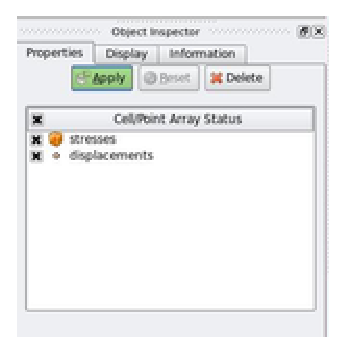
\includegraphics{snap6.eps}\\
		\vspace{0.5cm}
		\end{center}
		\item By default, \emph{surface} which is situated in the tool bar, is selected. You might prefer \emph{Surface with edges} that displays the mesh.\\
		\item If you want to see the displacements, switch \emph{Solid Color} in the tool bar to \emph{displacements}.\\
		\begin{center}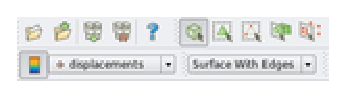
\includegraphics{snap7.eps}\\\end{center}
		\item On the left side of the main screen,\emph{Display} gives all the options to customize your screen. For instance, you can click on \emph{Edit Color Map} to display the legend.\\
		\begin{center}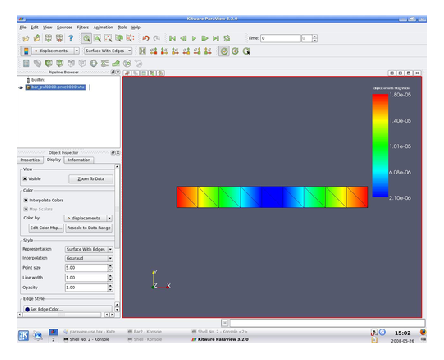
\includegraphics{snap2.eps}\\\end{center}
		\end{itemize}
	
	\item{Generate and read a movie}
		\begin{itemize}
		\item Type on your console \emph{generatePVD.pl directory bar >name\_movie.pvd} , where directory indicates the location of your vtu files. If you change one of you .vtu files, you don't need to recreate name\_movie.pvd.
		\item Open paraview. Open name\_movie.pvd. Don't forget to click on the green \emph{Apply} button.Choose the field you want to display, display the color map and play the movie).
		\item If you want to export the movie as a .avi file,
			\begin{itemize}
			\item first, generate a list of .jpg files using \textit{"Save animation"} in the File menu.
			\item then, use this command to turn the .jpg files into a .avi movie \textit{"mencoder "mf://*.jpg" -mf fps=6:type=jpg -ovc lavc -lavcopts vcodec=msmpeg4v2 -of avi -o movie.avi"}
			\end{itemize}
		\end{itemize}


	\end{enumerate}


\vspace{1.5cm}
These are the basics to generate paraview files and movie. If you are willing to improve your skills on paraview, you can refer to the User Manual book which is in our library!


\end{document}
